\section{Lebesgue and Sobolev Spaces}
For the abstract results on existence of solutions to the direct problem, \hyperlink{theorem_3_1_14}{Theorem 3.1.14} and \hyperlink{corollary_3_2_7}{Corollary 3.2.7}, we needed \textit{reflexive} Banach spaces. But the spaces of continuous, continuously differentiable or piecewise continuously differentiable functions aren't reflexive. For example, consider the bounded sequence $(u_n)_{n\in\mathbb{N}}\subset C^0([0,1])$ with
\[u_n:[0,1]\longrightarrow\mathbb{R},\qquad u_n(x):=\left\{\begin{array}{rl}
	1-nx&\text{if }x\in[0,1/n],\\
	0&\text{if }x\in(1/n,1].
\end{array}\right.\]

\begin{figure}[ht]
	\centering
	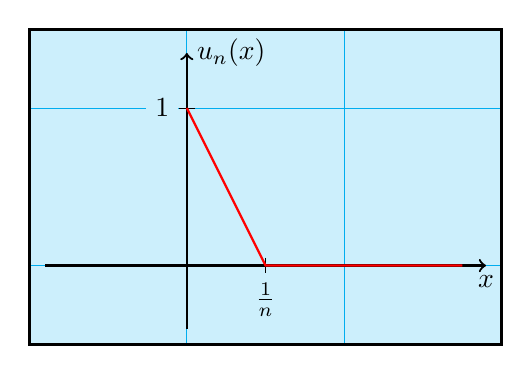
\begin{tikzpicture}
		% Hintergrund und Achsen
		\fill[cyan!20] (-2, -1) rectangle (4, 3);
		\draw[cyan, step=2] (-2, -1) grid (4, 3);
		\draw[thick, ->] (-1.8, 0) -- (3.8, 0) node[below] {$x$};
		\draw[thin] (0.1, 2) -- (-0.1, 2) node[left, fill=cyan!20] {1};
		\draw[thick, ->] (0, -0.8) -- (0, 2.7) node[right] {$u_n(x)$};
		\draw[thin] (1, 0.1) -- (1, -0.1) node[below] {$\frac{1}{n}$};
		\draw[very thick] (-2, -1) rectangle (4, 3);

		% Funktionen
		\draw[thick, red] (0, 2) -- (1, 0) -- (3.5, 0);
	\end{tikzpicture}
	\caption{Graph of $u_n$.}
\end{figure}

Then $\lVert u_n\rVert_{C^0([0,1])}=1$. For $x_0\in[0,1]$ consider the dirac measure
\[\delta_{x_0}:C^0([0,1])\longrightarrow\mathbb{R},\qquad\delta_{x_0}(u):=u(x_0).\]
This is linear and continuous, whence $\delta_{x_0}\in C^0([0,1])'$, and
\[\delta_{x_0}(u_n)=u_n(x_0)\to\left\{\begin{array}{rl}
	0&\text{if }x_0\in(0,1],\\
	1&\text{if }x_0=0.
\end{array}\right.\]
Hence, if a subsequence of $(u_n)_{n\in\mathbb{N}}$ would be weakly convergent, then the limit $u_*$ is
\[u_*(x)=\left\{\begin{array}{rl}
	1&\text{if }x=0,\\
	0&\text{if }x\in(0,1].
\end{array}\right.\]
However, $u_*\notin C^0([0,1])$, so $(u_n)_{n\in\mathbb{N}}$ has no weakly convergent subsequence. Hence, $C^0([0,1])$ cannot be reflexive by Eberlin-\v{S}mulian, \hyperlink{theorem_3_1_9}{Theorem 3.1.9}. In a same way, one can construct counterexamples for $C^1([0,1])$ and $PC^1([0,1])$.\\[33pt]

\paragraph{Lebesgue Spaces}
Let $\Omega\subset\mathbb{R}^d$ be open. A function $u:\Omega\longrightarrow\mathbb{R}$ is called \textit{measurable} if for all $a,b\in\mathbb{R}$ the preimage $u^{-1}([a,b))\subset\Omega$ is Lebesgue measurable. There are many other equivalent definitions for measurability. For $p\in[1,\infty)$, define
\[\lVert u\rVert_{L^p(\Omega)}:=\left(\int_\Omega{\lvert u(x)\rvert^p\mathrm{d}x}\right)^{1/p},\]
and for $p=\infty$ define
\[\lVert u\rVert_{L^\infty(\Omega)}:=\esssup_{x\in\Omega}{\lvert u(x)\rvert}=\inf\left\{\sup_{x\in\Omega\setminus N}{\lvert u(x)\rvert}\,\middle\vert\,N\subset\Omega\text{ null set }\right\}.\]
Let $\mathcal{L}^p(\Omega):=\{u:\Omega\longrightarrow\mathbb{R}\mid u\text{ is measurable with }\lVert u\rVert_{L^p(\Omega)}<\infty\}$. Then $\lVert\cdot\rVert_{L^p(\Omega)}$ is a seminorm on $\mathcal{L}^p(\Omega)$, and it becomes a norm on $L^p(\Omega):=\mathcal{L}^p(\Omega)/\sim$, where $u_1\sim u_2$ if $u_1(x)=u_2(x)$ for almost all $x\in\Omega$.\\

These objects, as well as the following list of properties for Lebesgue spaces, should already be known from \textit{Analysis} or \textit{Functional Analysis} course.
\begin{itemize}
	\item[(a)] For all $p\in[1,\infty]$ the pair $(L^p(\Omega),\lVert\cdot\rVert_{L^p(\Omega)})$ forms a Banach space.
	\item[(b)] We have some dense subsets:
	\begin{itemize}
		\item[(1)] The simple functions
		\[S(\Omega):=\operatorname{span}\{\chi_E:\Omega\longrightarrow\{0,1\}\mid E\subset\Omega\text{ measurable with finite measure}\}\]
		are dense in $L^p(\Omega)$ for all $p\in[1,\infty]$.
		\item[(2)] The smooth functions with compact support, i.e. $C_c^\infty(\Omega)$, are dense in $L^p(\Omega)$ for all $p\in[1,\infty)$.
	\end{itemize}
	\item[(c)] H\"older inequality: If $p,q\in[1,\infty]$ are such that $\frac{1}{p}+\frac{1}{q}=1$ and $u\in L^p(\Omega)$, $v\in L^q(\Omega)$, then
	\[\lVert u\cdot v\Vert_{L^1(\Omega)}\leq\lVert u\rVert_{L^p(\Omega)}\cdot\lVert v\Vert_{L^q(\Omega)}.\]
	In particular, if $\Omega$ is bounded, then $L^p(\Omega)\subset L^{\tilde{p}}(\Omega)$ for $p>\tilde{p}$.
	\item[(d)] For $p=2$, $L^2(\Omega)$ is a Hilbert space with scalar product
	\[\langle u,v\rangle=\int_\Omega{u(x)v(x)\mathrm{d}x}.\]
	\item[(e)] Riesz-Fischer representation theorem: Let $p\in[1,\infty)$ and $q\in(1,\infty]$ with $\frac{1}{p}+\frac{1}{q}=1$. Then $(L^p(\Omega))'$ is isometrically isomorphic to $L^q(\Omega)$: For every $\varphi\in(L^p(\Omega))'$ there exists a unique $v_\varphi\in L^q(\Omega)$ such that
	\[\varphi(u)=\int_\Omega{u(x)v_\varphi(x)\mathrm{d}x}\]
	for all $u\in L^p(\Omega)$, and $\lVert\varphi\rVert_{(L^p(\Omega))'}=\lVert v_\varphi\rVert_{L^q(\Omega)}$. In particular, $(L^p(\Omega))''=L^p(\Omega)$ for $p\in(1,\infty)$ and hence $L^p(\Omega)$ is reflexive if $p\in(1,\infty)$.
	\item[(f)] One the one hand we have $(L^1(\Omega))'\simeq L^\infty(\Omega)$, but $L^1(\Omega)$ is a proper subspace of $(L^\infty(\Omega))'$ in general, so that $L^p(\Omega)$ is not reflexive for $p\in\{1,\infty\}$.
	\item[(g)] Characterization of weak convergence in $L^p(\Omega)$ for $p\in(1,\infty)$: A sequence $(u_n)_{n\in\mathbb{N}}\subset L^p(\Omega)$ converges weakly to $u\in L^p(\Omega)$ in $L^p(\Omega)$ if and only if $\lVert u_n\rVert_{L^p(\Omega)}\leq C$ and for all $\varphi\in C_c^\infty(\Omega)$ it holds
	\[\int_\Omega{u_n(x)\varphi(x)\mathrm{d}x}\to\int_\Omega{u(x)\varphi(x)\mathrm{d}x}.\]
	We can also replace $C_c^\infty(\Omega)$ by $S(\Omega)$, and thanks to linearity of the integral we can even reduce the test-functions to characteristic functions which then is just integration over subsets.\\[11pt]
\end{itemize}

\textbf{\underline{Definition 3.3.1}}\\
(Weak derivative)\\
Let $u\in L_\text{loc}^1(\Omega):=\{u:\Omega\longrightarrow\mathbb{R}\mid u|_\omega\in L^1(\omega)\text{ for all }\omega\subset\mathrel\subset\Omega\}$, where $\omega\subset\mathrel\subset\Omega$ means that $\omega$ is a compact subset of $\Omega$. Let $\alpha=(\alpha_1,\dotsc,\alpha_d)\in\mathbb{N}_0^d$ be a multi-index. A function $v_\alpha\in L_\text{loc}^1(\Omega)$ is called an \textit{$\alpha$-th weak derivative of $u$} if
\[\int_\Omega{u(x)D^\alpha\varphi(x)\mathrm{d}x}=(-1)^{\lvert\alpha\rvert}\int_\Omega{v_\alpha(x)\varphi(x)\mathrm{d}x}\]
for all $\varphi\in C_c^\infty(\Omega)$, where $\lvert\alpha\rvert:=\sum_{i=1}^d{\alpha_i}$ and $D^\alpha\varphi=\frac{\partial^{\lvert\alpha\rvert}\varphi}{\partial x_1^{\alpha_1}\cdots\partial x_d^{\alpha_d}}$. We set $D^\alpha u:=v_\alpha$. This is justified by \hyperlink{remark_3_3_2}{Remark 3.3.2 (b)}.\\[11pt]

\hypertarget{remark_3_3_2}{\textbf{Remark 3.3.2}}
\begin{itemize}
	\item[(a)] If $u$ is differentiable in the classical sense, then the weak derivative coincides with the classical derivative.
	\item[(b)] The weak derivative is unique. So, if $v_\varphi$ and $w_\varphi$ are $\alpha$-th weak derivatives of $u$, then
	\[\int_\Omega{v_\alpha(x)\varphi(x)\mathrm{d}x}=(-1)^{\lvert\alpha\rvert}\int_\Omega{u(x)D^\alpha\varphi(x)\mathrm{d}x}=\int_\Omega{w_\alpha(x)\varphi(x)\mathrm{d}x}\]
	for all $\varphi\in C_c^\infty(\Omega)$. Therefore, $\int_\Omega{(v_\alpha(x)-w_\alpha(x))\varphi(x)\mathrm{d}x}=0$ for all $\varphi\in C_c^\infty(\Omega)$, so $v_\alpha-w_\alpha=0$ almost everywhere by the fundamental lemma of calculus of variations (in a version for locally integrable functions).\\[11pt]
\end{itemize}

\textbf{Example 3.3.3}\\
Let $u:\mathbb{R}\longrightarrow\mathbb{R}$, $u(x):=\lvert x\rvert$. Then $u$ is continuous, but not (classically) differentiable in 0. But $u$ is weakly differentiable, and we want to compute its weak derivative. We would expect that the weak derivative coincides (almost everywhere) on the set of points where $u$ is classically differentiable. So, we would expect that the weak derivative is $v(x)=\sgn{x}$ for $x\ne0$, and it doesn't matter how $v$ is defined at zero because pointwise it is only defined almost everywhere. For $\varphi\in C_c^\infty(\mathbb{R})$, integration by parts yields
\begin{align*}
	\int_\mathbb{R}{u(x)\varphi'(x)\mathrm{d}x}&=\int_{-\infty}^0{-x\varphi'(x)\mathrm{d}x}+\int_0^\infty{x\varphi'(x)\mathrm{d}x}\\
	&=-0\cdot\varphi(0)+\lim_{x\to-\infty}{(-x\varphi(x))}+\int_{-\infty}^0{1\cdot\varphi(x)\mathrm{d}x}\\
	&\qquad\qquad+\lim_{x\to+\infty}{x\varphi(x)}-0\cdot\varphi(0)-\int_0^\infty{1\cdot\varphi(x)\mathrm{d}x}\\
	&=-\int_\mathbb{R}{\sgn{x}\varphi(x)\mathrm{d}x}=-\int_\mathbb{R}{v(x)\varphi(x)\mathrm{d}x}.
\end{align*}
Hence, $v$ is the weak derivative of $u$, i.e. $u'=v$ in the weak sense.\\

We can ask further if $v$ is weakly differentiable. It is not continuous at 0, but on $\mathbb{R}\setminus\{0\}$ this function is infinitely many often differentiable. If $v$ would be weakly differentiable, then its weak derivative $w=v'$ would satisfy
\begin{align*}
	-\int_\mathbb{R}{w(x)\varphi(x)\mathrm{d}x}&=\int_\mathbb{R}{v(x)\varphi'(x)\mathrm{d}x}\\
	&=\int_{-\infty}^0{-\varphi'(x)\mathrm{d}x}+\int_0^\infty{\varphi'(x)\mathrm{d}x}\\
	&=-\varphi(0)+\lim_{x\to-\infty}{\varphi(x)}+\lim_{x\to+\infty}{\varphi(x)}-\varphi(0)=-2\varphi(0)
\end{align*}
for all $\varphi\in C_c^\infty(\mathbb{R})$. This would mean that $w$ represents a Dirac measure which is impossible for an $L_\text{loc}^1(\mathbb{R})$-function. Therefore, $v$ is \textit{not} weakly differentiable.\\[11pt]

\textbf{\underline{Definition 3.3.4}}\\
(Sobolev space)\\
Let $\Omega\subset\mathbb{R}^d$ be open, $p\in[1,\infty]$, $k\in\mathbb{N}$. Define
\[W^{k,p}(\Omega):=\left\{u\in L^p(\Omega)\,\middle\vert\,\begin{array}{c}
	\text{For all }\alpha\in\mathbb{N}_0^d\text{ with }\lvert\alpha\rvert\leq k,\text{ the weak}\\
	\text{derivative }D^\alpha u\text{ exists and }D^\alpha u\in L^p(\Omega).
\end{array}\right\}\]
with norm
\[\lVert u\rVert_{W^{k,p}(\Omega)}:=\left(\sum_{\alpha\in\mathbb{N}_0^d,\lvert\alpha\rvert\leq k}{\lVert D^\alpha u\rVert_{L^p(\Omega)}^p}\right)^{1/p}\]
if $p<\infty$, and
\[\lVert u\rVert_{W^{k,\infty}(\Omega)}:=\max\left\{\lVert D^\alpha u\rVert_{L^\infty(\Omega)}\,\middle\vert\,\alpha\in\mathbb{N}_0^d,\lvert\alpha\rvert\leq k\right\}.\]
The definition makes sense because $L^p(\Omega)\subset L_\text{loc}^1(\Omega)$.\\

Moreover, we set $W_0^{k,p}(\Omega):=\overline{C_c^\infty(\Omega)}^{W^{k,p}(\Omega)}$, i.e. $W_0^{k,p}(\Omega)$ is the closure of $C_c^\infty(\Omega)$ in $W^{k,p}(\Omega)$ with respect to norm $\lVert\cdot\rVert_{W^{k,p}(\Omega)}$. We also abbreviate $H^k(\Omega):=W^{k,2}(\Omega)$.\\[11pt]

\textbf{Remark 3.3.5}\\
(most important properties of Sobolev spaces)\\
The following can be looked up in the literature, for instance in \cite[Chapter 3 ??]{adams_fournier} or \cite[Part II, 5. Sobolev Spaces]{lawrence_evans}.
\begin{itemize}
	\item[(a)] $(W^{k,p}(\Omega),\lVert\cdot\rVert_{W^{k,p}(\Omega)})$ is a Banach space for all $p\in[1,\infty]$, $k\in\mathbb{N}_0$.
	\item[(b)] $(H^k(\Omega),\langle\cdot,\cdot\rangle_k)$ are Hilbert spaces with scalar product
	\[\langle u,v\rangle_k:=\sum_{\alpha\in\mathbb{N}_0^d,\lvert\alpha\rvert\leq k}{\langle D^\alpha u,D^\alpha v\rangle_{L^2(\Omega)}}.\]
	\item[(c)] $W_0^{k,p}(\Omega)$ is a Banach space.
	\item[(d)] For $p\in(1,\infty)$, the dual space of $W^{k,p}(\Omega)$ is isomorphic to $W^{k,q}(\Omega)$, where $\frac{1}{p}+\frac{1}{q}=1$. More precisely, for all $\varphi\in(W^{k,p}(\Omega))'$ there is a unique $w\in W^{k,q}(\Omega)$ such that for all $u\in W^{k,p}(\Omega)$ we have
	\[\varphi(u)=\sum_{\alpha\in\mathbb{N}_0^d,\lvert\alpha\vert\leq k}{\int_\Omega{D^\alpha u(x)D^\alpha w(x)\mathrm{d}x}}.\]
	In particular, $W^{k,p}(\Omega)$ is reflexive for $p\in(1,\infty)$. This is in the same spirit as for the Lebesgue spaces.
	\item[(e)] For $p\in[1,\infty)$, a sequence $(u_n)_{n\in\mathbb{N}}\subset W^{k,p}(\Omega)$ converges weakly to $u\in W^{k,p}(\Omega)$ if and only if $D^\alpha u_n\rightharpoonup D^\alpha u$ in $L^p(\Omega)$ as $n\to\infty$ for all $\alpha\in\mathbb{N}_0^d$ with $\lvert\alpha\rvert\leq k$.
	\item[(f)] For $p\in[1,\infty)$,
	\begin{itemize}
		\item[(1)] $W^{k,p}(\Omega)\cap C^\infty(\Omega)$ is dense in $W^{k,p}(\Omega)$;
		\item[(2)] $C^\infty(\overline{\Omega})=\{v|_\Omega\mid v\in C^\infty(\mathbb{R}^d)\}$ is dense in $W^{k,p}(\Omega)$ if $\Omega\subset\mathbb{R}^d$ is a bounded domain with Lipschitz boundary (i.e. $\partial\Omega$ is locally the graph of a Lipschitz continuous function).
	\end{itemize}
	\item[(g)] If $\Omega\subset\mathbb{R}^d$ is bounded, then $W^{1,\infty}(\Omega)$ is isomorphic to the space of Lipschitz continuous functions.
	\item[(h)] In general, $W_0^{k,p}(\Omega)\subsetneq W^{k,p}(\Omega)$. However, $W_0^{k,p}(\mathbb{R}^d)=W^{k,p}(\mathbb{R}^d)$ if $p<\infty$.\\[11pt]
\end{itemize}

We further need embedding theorems for Sobolev spaces. Here, the Sobolev number $k^*:=k-\frac{d}{p}$ plays a crucial role, where as before $k$ denotes the order of differentiability, $p$ the order of integrability and $d$ the dimension.\\

To understand where this number comes from, we look as a motivation at $\Omega=(0,1)$, $u_a(x)=x^a$ for some $a\in\mathbb{R}$. It depends on $a$ (especially when $a<0$) if $u_a\in L^p(\Omega)$ for some $p$. When do we have $u_a\in W^{k,p}(0,1)$? One can show that the crucial point somehow is the highest order derivative, so $u_a\in W^{k,p}(0,1)$ if and only if
\[\int_0^1{\lvert u_a^{(k)}(x)\rvert^p\mathrm{d}x}=\int_0^1{x^{(a-k)p}\mathrm{d}x}<\infty.\]
This is finite if $(a-k)p>-1$, i.e. if $a>k-\frac{1}{p}=k^*$ for ($d=1$). Similarly on can show $(x\mapsto\lvert x\rvert^a)\in W^{k,p}((0,1)^d)$ if and only if $a>k-\frac{d}{p}=k^*$.\\[11pt]

\textbf{\underline{Definition 3.3.6}}\\
(H\"older space)\\
Let $\Omega\subset\mathbb{R}^d$ be open and bounded. A function $u:\Omega\longrightarrow\mathbb{R}$ is called \textit{H\"older continuous} for exponent $\gamma\in(0,1]$ if
\[[u]_\gamma:=\sup\left\{\frac{\lvert u(x)-u(y)\rvert}{\lvert x-y\rvert^\gamma}\,\middle\vert\,x,y\in\Omega,x\ne y\right\}<\infty.\]
For $k\in\mathbb{N}_0$, we define the space
\[C^{k,\gamma}(\overline{\Omega}):=\left\{u\in C^k(\overline{\Omega})\,\middle\vert\,[D^\alpha u]_\gamma<\infty\text{ for all }\alpha\in\mathbb{N}_0^d,\lvert\alpha\rvert\leq k\right\},\]
endowed with the norm
\[\lVert u\rVert_{C^{k,\gamma}(\overline{\Omega})}:=\sum_{\alpha\in\mathbb{N}_0^d,\lvert\alpha\rvert\leq k}{\lVert D^\alpha u\rVert_{C^0(\overline{\Omega})}}+\sum_{\alpha\in\mathbb{N}_0^d,\lvert\alpha\rvert=k}{[D^\alpha u]_\gamma}.\]\\
	
\textbf{Remark 3.3.7}\\
One can show that $(C^{k,\gamma}(\overline{\Omega}),\lVert\cdot\rVert_{C^{k,\gamma}(\overline{\Omega})})$ is a Banach space, but it is not reflexive. Also note that the norm is formed with the $C^0$-norms over all derivatives, while the sum over $[D^\alpha u]_\gamma$ is only taken over the derivatives of order $k$.\\[11pt]

\textbf{\underline{Definition 3.3.8}}\\
Let $(X,\lVert\cdot\rVert_X)$, $(Y,\lVert\cdot\rVert_Y)$ be normed spaces and $X\subseteq Y$. We say that \textit{$X$ embeds continuously (compactly) into $Y$} if the identical embedding $\iota:X\longrightarrow Y$, $x\longmapsto x$, is a continuous (compact) operator.\\

For continuous embeddings we write $X\longhookrightarrow Y$, and for compact embeddings $X\clonghookrightarrow Y$.\\[11pt]

\textbf{Remark 3.3.9}
\begin{itemize}
	\item[(a)] $X$ embeds continuously into $Y$ if there exists $C>0$ such that $\lVert x\rVert_Y\leq C\lVert x\rVert_X$ for all $x\in X$.
	\item[(b)] $X$ embeds compactly into $Y$ if every weakly convergent sequence in $X$ converges strongly in $Y$, i.e. if $(u_n)_{n\in\mathbb{N}}\subset X$, $u\in X$, then $u_n\rightharpoonup u$ in $X$ implies $u_n\to u$ in $Y$.\\[11pt]
\end{itemize}

\hypertarget{theorem_3_3_10}{\textbf{\underline{Theorem 3.3.10}}}\\
(Sobolev embedding theorem)\\
Let $\Omega\subset\mathbb{R}^d$ be a (not necessarily bounded) domain with Lipschitz boundary $\partial\Omega$. Let $\tilde{k},k\in\mathbb{N}_0$ with $k\geq\tilde{k}$.
\begin{itemize}
	\item[(i)] If $p,\tilde{p}\in[1,\infty)$ with $\tilde{p}\geq p$ and $k-\frac{d}{p}\geq\tilde{k}-\frac{d}{\tilde{p}}$, then $W^{k,p}(\Omega)\longhookrightarrow W^{\tilde{k},\tilde{p}}(\Omega)$.
	\item[(ii)] If $p\in[1,\infty)$ and $\gamma\in(0,1)$ are such that $k-\frac{d}{p}\geq\tilde{k}+\gamma$, then $W^{k,p}(\Omega)\longhookrightarrow C^{\tilde{k},\gamma}(\overline{\Omega})$.\\
\end{itemize}

\textit{Proof:}\\
This is treated in the course \textit{Partial Differential Equations}, but the proof can also be looked up in appropriate literature, e.g. \cite[Kapitel 8, 8.9 Einbettungssatz in Sobolev-R\"aumen, 8.13 Einbettungssatz von Sobolev-R\"aumen in H\"older-R\"aume]{hans_wilhelm_alt} for bounded domains.\hfill$\blacksquare$\\[11pt]

\textbf{\underline{Theorem 3.3.11}}\\
(Rellich compactness theorem)\\
If $\Omega\subset\mathbb{R}^d$ is a \textit{bounded} domain with Lipschitz boundary, and if we have strict inequalities in \hyperlink{theorem_3_3_10}{Theorem 3.3.10}, i.e. $k-\frac{d}{p}>\tilde{k}-\frac{d}{p}$ or $k-\frac{d}{p}>\tilde{k}+\gamma$, then the above embeddings are compact.\\

\textit{Proof:}\\
As before, we refer to the literature.\hfill$\blacksquare$\\[11pt]

\textbf{Examples 3.3.12}
\begin{itemize}
	\item[(a)] Consider $k=1$, $p=2$.
	\begin{itemize}
		\item[(1)] If $d=1$, then the Sobolev number is $1-\frac{1}{2}=\frac{1}{2}$. So in case (i), for $\tilde{k}=0$ we can choose any $\tilde{p}\in[2,\infty)$ to obtain an embedding $H^1(\Omega)\longhookrightarrow L^{\tilde{p}}(\Omega)$, and in (ii) we have $H^1(\Omega)\longhookrightarrow C^{0,\gamma}(\overline{\Omega})$ for $\gamma\leq\frac{1}{2}$.
		\item[(2)] If $d=2$, then the Sobolev number is $1-\frac{2}{2}=0$. So case (ii) is no longer applicable, but we still have $H^1(\Omega)\longhookrightarrow L^{\tilde{p}}(\Omega)$ for $\tilde{p}\in[2,\infty)$.
		\item[(3)] If $d=3$, the then Sobolev number is $1-\frac{3}{2}=-\frac{1}{2}$. This gives $H^1(\Omega)\longhookrightarrow L^{\tilde{p}}(\Omega)$ for $\tilde{p}\in[2,6]$.
	\end{itemize}
	If $\Omega$ is bounded, the embeddings $H^1(\Omega)\longhookrightarrow L^{\tilde{p}}(\Omega)$ also hold for $\tilde{p}\in[1,2)$ by H\"older's inequality.
	\item[(b)] For $k=1$ and $p\in[1,\infty)$, we have the continuous embedding $W^{1,p}(\Omega)\longhookrightarrow L^{\tilde{p}}(\Omega)$ for
	\begin{itemize}
		\item[(1)] $p<d$ and $p\leq\tilde{p}\leq\frac{dp}{d-p}$,
		\item[(2)] $p=d$ and $p\leq\tilde{p}<\infty$,
		\item[(3)] $p>d$ and $p\leq\tilde{p}\leq\infty$. (Infinity via the embedding $C^{0,\gamma}(\overline{\Omega})\longhookrightarrow C^0(\overline{\Omega})\longhookrightarrow L^\infty(\Omega)$.)
	\end{itemize}
	If we have $p>d$, we further have $W^{1,p}(\Omega)\longhookrightarrow C^{0,\gamma}(\overline{\Omega})$ with $\gamma\leq1-\frac{d}{p}$.\\

	These embeddings are compact if $\Omega$ is bounded and if $\tilde{p}<\frac{dp}{d-p}$ in case $p<d$, or if $\gamma<1-\frac{d}{p}$ in case $p>d$. In particular, if $u_n\rightharpoonup u_*$ in $W^{1,p}(\Omega)$ for some $(u_n)_{n\in\mathbb{N}}\subset W^{1,p}(\Omega)$ and $u_*\in W^{1,p}(\Omega)$, then
	\begin{itemize}
		\item[(i)] $u_n\to u_*$ in $L^{\tilde{p}}(\Omega)$ if $\tilde{p}<d$ and $\frac{1}{\tilde{p}}>\frac{1}{p}-\frac{1}{d}$,
		\item[(ii)] $u_n\to u$ in $C^0(\overline{\Omega})$ if $p>d$, i.e. uniform convergence.\\[11pt]
	\end{itemize}
\end{itemize}

In \hyperref[chap:mcov_chap2]{Chapter II. Classical Methods}, functionals were defined on classes of functions $u$ with prescribed boundary values $u|_{\Gamma_D}$ with $\Gamma_D\subset\partial\Omega$. Since $\Gamma_D$ has Lebesgue measure zero, the expression $u|_{\Gamma_D}$ does not make sense for $u\in L^p(\Omega)$. However, for Sobolev functions $u$, there is a notion of so-called ``trace'' $u|_{\partial\Omega}$.\\

\textbf{\underline{Theorem 3.3.13}}\\
(Trace theorem)\\
Let $\Omega\subset\mathbb{R}^d$ be a bounded domain with Lipschitz boundary, and let $p,q\in[1,\infty]$ such that
\[\left\{\begin{array}{rl}
	q<\frac{(d-1)p}{d-p}&\text{if }p<d,\\
	q<\infty&\text{if }d=p,\\
	q\leq\infty&\text{if }p>d.
\end{array}\right.\]
(In particular, $q=p$ is allowed in all three cases.) Then the operator $C^1(\overline{\Omega})\longrightarrow C^0(\partial\Omega)$, $u\longmapsto u|_{\partial\Omega}$ has a unique extension to a bounded linear operator $\gamma:W^{1,p}(\Omega)\longrightarrow L^q(\partial\Omega)$, called \textit{trace operator}, where $\partial\Omega$ is equipped with surface measure. This means, $\gamma$ is a bounded linear operator with $\gamma(u)=u|_{\partial\Omega}$ for all $u\in C^1(\overline{\Omega})$.\\

\textit{Proof:}\\
As before, this is treated in \textit{Partial Differential Equations} in detail, but can be looked up in the literature as well.\hfill$\blacksquare$\\[11pt]

\textbf{Remark 3.3.14}\\
If $\Omega\subset\mathbb{R}^d$ is a bounded Lipschitz domain, then $\{u\in W^{1,p}(\Omega)\mid\gamma(u)=0\}=W_0^{1,p}(\Omega)$.\\[11pt]

\textbf{\underline{Theorem 3.3.15}}\\
(Poincar\'e's inequality)\\
Let $\Omega\subset\mathbb{R}^d$ be open and bounded, $p\in[1,\infty)$. Then for all $u\in W_0^{1,p}(\Omega)$ it holds
\[\lVert u\rVert_{L^p(\Omega)}\leq\diam{\Omega}\lVert\nabla u\rVert_{L^p(\Omega;\mathbb{R}^d)},\]
where $\diam{\Omega}:=\sup\{\lvert x-y\rvert:x,y\in\Omega\}$.\\

\textit{Proof:}\\
Since $C_c^\infty(\Omega)$ is dense in $W_0^{1,p}(\Omega)$ by definition, it suffices to consider $u\in C_c^\infty(\Omega)$ instead of $u\in W_0^{1,p}(\Omega)$. Let $\delta:=\diam{\Omega}$, and extend $u$ by zero to $\mathbb{R}^d$. For $x\in\Omega$ we obtain
\[u(x)=u(x)-u(x-\delta e_1)=\int_0^1{\frac{\mathrm{d}}{\mathrm{d}s}[u(x-(1-s)\delta e_1)]\mathrm{d}s}=\int_0^1{\delta\partial_1u(x-(1-s)\delta e_1)\mathrm{d}s},\]
hence, by H\"older's inequality,
\begin{align*}
	\lvert u(x)\rvert^p&\leq\delta^p\left(\left(\int_0^1{1^{p'}\mathrm{d}x}\right)^{1/p'}\left(\int_0^1{\lvert\partial_1u(x-(1-s)\delta e_1)\rvert^{p}\mathrm{d}s}\right)^{1/p}\right)^p\\
	&\leq\delta^p\int_0^1{\lvert\nabla u(x-(1-s)\delta e_1)\rvert^p\mathrm{d}s}.
\end{align*}
Integrating over $\Omega$ yields, together with Fubini,
\begin{align*}
	\int_\Omega{\lvert u(x)\rvert^p\mathrm{d}x}&\leq\delta^p\int_0^1{\int_\Omega{\lvert\nabla u(x-(1-s)\delta e_1)\rvert^p\mathrm{d}x}\mathrm{d}s}\\
	&\leq\delta^p\int_0^1{\int_\Omega{\lvert\nabla u(y)\rvert^p\mathrm{d}y}\mathrm{d}s}\\
	&=\delta^p\int_\Omega{\lvert\nabla u(y)\rvert^p\mathrm{d}y}.
\end{align*}
\hfill$\blacksquare$\\[11pt]

\textbf{Remark 3.3.16}
\begin{itemize}
	\item[(a)] The proof can be changed by choosing another $i$-th unit vector than $e_1$. That's why one could expect that Poincar\'e's inequality even hold true for more general domains, e.g., if $\Omega$ lies between two hyperplanes. So in particular, $\Omega$ could be unbounded. Indeed, one can adapt this proof for such domains, but then the constant $\diam{\Omega}$ has to be changed to a certain distance between the hyperplanes.
	\item[(b)] Poincar\'e's inequality shows
	\[\lVert\nabla u\rVert_{L^p(\Omega;\mathbb{R}^d)}\leq\lVert u\rVert_{W^{1,p}(\Omega)}\leq\diam{\Omega}\lVert\nabla u\rVert_{L^p(\Omega;\mathbb{R}^d)}\]
	for all $u\in W_0^{1,p}(\Omega)$. This means that $\lVert\cdot\rVert_{W^{1,p}(\Omega)}$ and $\lVert\nabla(\cdot)\rVert_{L^p(\Omega;\mathbb{R}^d)}$ are equivalent norms on $W_0^{1,p}(\Omega)$.
\end{itemize}
\leavevmode